\documentclass[10pt]{beamer}
\usetheme{metropolis}  
\usecolortheme{beaver}
\usepackage{hyperref}
\usepackage{bigints}
\usepackage{amsmath}
\usepackage{verbatim}
\title{Introducci\'on a la probabilidad y estad\'istica CM274}
 \usepackage[spanish]{babel}
\date{\today}
\author{C\'esar Lara Avila}
\institute{\url{https://github.com/C-Lara}}
\begin{document}
  \maketitle
  \section{4. Variables aleatorias discretas }
  
\begin{frame}{Variables aleatorias}
Este tema trata en gran medida de introducir alguna terminolog\'ia \'util, bas\'andose en las nociones de espacio muestral y funci\'on de probabilidad. Las palabras clave son:

\begin{enumerate}
	\item Variable aleatoria.
	\item Funci\'on de masa de probabilidad (PMF).
	\item Funci\'on de distribuci\'on acumulativa (CDF).
\end{enumerate}

\vspace{0.2cm}

\textbf{\small{\underline{Recordar:}}}
\begin{itemize}
	\item \scriptsize{Un espacio muestral discreta $\Omega$ es finito o es un conjunto listable de salidas $\{\omega_1, \omega_2, \dots\}$. La probabilidad de una salida $\omega$ es denotada por $\mathbb{P}(\omega)$}.
	\item Un evento $E$ es un subconjunto de $\Omega$. La probabilidad de un evento $E$ es
	
	\[
	 \mathbb{P}(E) = \sum_{\omega \in E}\mathbb{P}(\omega).
	 \]
\end{itemize}
\end{frame}
 \begin{frame}{Ejemplo de variables aleatorias}
\begin{itemize}
	\item \small {\textbf{Ejemplo 1} Un juego  con $2$ dados.
	
	Tirar un dado dos veces y registrar los resultados como $(i, j)$, donde $i$ es el resultado de la primera tirada y $j$ el resultado de la segunda. Podemos tomar el espacio muestral:
	
	\[
	\Omega =\{ (1,1),(1,2),(1, 3), \dots, (6,6)\} = \{(i,j)|i,j = 1, \dots, 6\}.
	\]
	
La funci\'on de probabilidad  es $\mathbb{P}(i,j) = 1/36$. 	

\vspace{0.2cm}

En este juego, tu ganas $500$ soles si la suma es $7$ y perdemos $100$ en otro caso. Damos a esta funci\'on de pago (payoff) el nombre de $X$, que describe esto formalmente como:

\[
X_{i,j} = \begin{cases}
500 & \text{si}\ i + j = 7\\
-100 & \text{si}\ i + j \neq 7.
\end{cases}
\]
}
\end{itemize}
\end{frame}
\begin{frame}{Ejemplo de variables aleatorias(1)}
\begin{itemize}
\item \small {\textbf{Ejemplo 2}
	
Podemos cambiar el juego usando una funci\'on de pago diferente. Por ejemplo:

\vspace{0.2cm}

\[
Y(i,j) = ij -10.
\]

\vspace{0.2cm}

En este ejemplo, si tira $(6, 2)$ entonces gana  $2$ soles. Si tira $(2, 3)$ entonces ganas  $-4$ (es decir, pierdes $4$ soles).

\vspace{0.2cm}

\textbf{\small{\underline{Pregunta:}}}
?`Qu\'e juego es la mejor apuesta?.

\vspace{0.5cm}


\textbf{\small{\underline{Observaci\'on importante :}}}

\vspace{0.2cm}

\textcolor{orange}{Las variables aleatorias asignan un n\'umero a cada salida en un espacio muestral.}
}	
\end{itemize}	
\end{frame}

\begin{frame}{Definici\'on }
Sea $\Omega $ un espacio muestral. Una \textbf{\textcolor{brown}{variable aleatoria discreta}} es una funci\'on:

\[
X: \Omega \rightarrow \mathbb{R}
\]

que toma un conjunto de valores discretos.

\vspace{0.2cm}

\small{\underline{?`Por qu\'e se llama $X$ a una variable aleatoria?}


Es \texttt{aleatoria} porque su valor depende de un resultado aleatorio de un experimento. Y tratamos a $X$ como lo har\'iamos con una variable usual: podemos a\~nadirla a otras variables aleatorias, elevarla al cuadrado y as\'i sucesivamente.}
\end{frame}

\begin{frame}{Definici\'on(1) }
\small{Dado un experimento y el correspondiente conjunto de posibles respuestas o salidas (el espacio muestral), una variable aleatoria asocia un n\'umero particular con cada respuestas o salidas, como se indica en la figura siguiente:} 


\vspace{0.2cm}


\begin{figure}[ht]
	\centering
	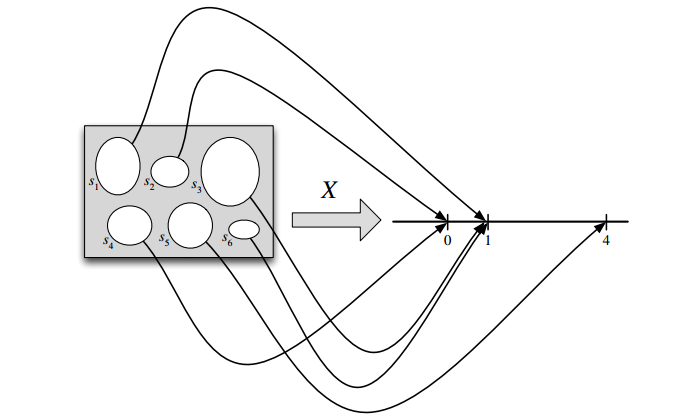
\includegraphics[width=6cm]{v1}
\end{figure}

\small{donde la variable aleatoria $X$ representada, es definida sobre un espacio muestral con $6$ elementos y los valores posibles $1, 2$ y $4$. La aleatoriedad viene de la elecci\'on de un punto  aleatorio de acuerdo con la funci\'on de probabilidad $\mathbb{P}$ para el espacio muestral.}
\end{frame}

\begin{frame}{Eventos y variables aleatorias }
Para alg\'un valor $a$, escribimos $X = a$, para indicar que el evento  consiste de todas las salidas $\omega$ con $X(\omega) = a$.

\begin{itemize}
\item \small {\textbf{Ejemplo 3} 
	
En el Ejemplo 1, lanzamos dos dados y $X$ fue una variable aleatoria

\[
X_{i,j} = \begin{cases}
500 & \text{si}\ i + j = 7\\
-100 & \text{si}\ i + j \neq 7.
\end{cases}
\]

El evento $X = 500$ es el conjunto $\{(1,6), (2,5), (3,4), (4,3), (5,2), (6,1) \}$, esto es, el conjunto de todas las salidas que suman $7$. As\'i $\mathbb{P}(X = 500) = 1/6$.
}
\end{itemize}

\vspace{0.2cm}

\scriptsize{Permitimos que $a$ sea un valor, incluso valores que $X$ nunca toma. En el ejemplo $1$, podr\'iamos mirar el evento $X = 1000$. Puesto que $X$ nunca es igual a $1000$ esto es solo el evento vac\'io (o conjunto vac\'io). }
\end{frame}

\begin{frame}{Funci\'on de masa de probabilidad }
	
Resulta dif\'icil de leer y escribir $\mathbb{P}(X = a)$ para la probabilidad  que $X = a$. Cuando sabemos que estamos hablando de X simplemente escribiremos $p(a)$. Si queremos hacer expl\'icita  $X$ escribiremos $p_X(a)$.
	
Explicamos esto con  una definici\'on.

\vspace{0.2cm}

\textbf{\small{\underline{Definici\'on:}}} \textcolor{blue}{La funci\'on de masa de probabilidad (PMF)} de una variable aleatoria discreta es la funci\'on $p(a) = \mathbb{P}(X =a)$. Se debe notar que:

\begin{itemize}
	\item Siempre se tiene $0 \leq p(a)\leq 1$.
	\item Permitimos que $a$ sea un n\'umero. Si $a$ es un valor que no toma $X$, entonces $p(a) = 0$.
\end{itemize}

\end{frame}

\begin{frame}{Ejemplo explicativo}

\begin{itemize}
\item \small {\textbf{Ejemplo 4}
Sea $\Omega$ el espacio muestral anterior de tirar $2$ dados. Definamos la variable aleatoria $M$ como el valor m\'aximo de los dos dados:

\[
M(i,j) = \max(i, j).
\]

Podemos describir una variable aleatoria enumerando sus posibles valores y las probabilidades asociadas a estos valores. Para el ejemplo anterior tenemos:

\vspace{0.2cm}

\begin{table}[]
	\centering
	\begin{tabular}{ccccccc}
		valor  a:    & 1    & 2    & 3    & 4    & 5    & 6     \\
		PMF    p(a): & 1/36 & 3/36 & 5/36 & 7/36 & 9/36 & 11/36
	\end{tabular}
\end{table}

\vspace{0.2cm}

Por ejemplo $p(2) = 3/36$.
}
\end{itemize}
\end{frame}

\begin{frame}{Eventos y desigualdades}
Las desigualdades con variables aleatorias describen eventos. Por ejemplo, $X \leq  a$ es el conjunto de todos los resultados $\omega$ tales que $X(\omega) \leq a$.

\vspace{0.5cm}

\begin{itemize}
	\item \small {\textbf{Ejemplo 5}

Si el espacio muestral es el conjunto de todos los pares de $(i, j)$ procedentes de tirar dos dados y $Z(i, j) = i + j$ es la suma de los dados entonces:

\[
Z \leq 4 = \{(1, 1), (1, 2), (1, 3), (2, 1), (2, 2), (3, 1) \}
\]
	}
\end{itemize}
\end{frame}
\begin{frame}{Funci\'on de distribuci\'on acumulativa}
\textbf{\small{\underline{Definici\'on:}}} \textcolor{blue}{ La funci\'on de distribuci\'on acumulativa (CDF)} de una variable aleatoria $X$ es la funci\'on $F$ dada por $F(a) = \mathbb{P}(X \leq a)$. Con frecuencia acortaremos esto a la \textcolor{blue}{funci\'on de distribuci\'on}.

Tenga en cuenta que la definici\'on de $F(a)$ usa el s\'imbolo menor o igual. Esto ser\'a importante para obtener los c\'alculos exactamente .


\begin{itemize}
\item \small {\textbf{Ejemplo 6} Continuando con el ejemplo $M$, tenemos:
		
\begin{table}[]
	\centering
	\begin{tabular}{ccccccc}
		valor a:   & 1    & 2    & 3    & 4    & 5    & 6     \\
		PMF   p(a): & 1/36 & 3/36 & 5/36 & 7/36 & 9/36 & 11/36 \\
		CDF   F(a): & 1/36 & 4/36 & 9/36 & 16/36 & 25/36 & 36/36	
	\end{tabular}
\end{table}
}
\end{itemize}

\vspace{0.3cm}

\scriptsize{$F(a)$ se denomina funci\'on de distribuci\'on acumulativa porque $F(a)$ da la probabilidad total que se acumula sumando las probabilidades $p(b)$ cuando $b$ va de $-\infty$ a $a$.
	
Por ejemplo, en la tabla anterior, la entrada $16/36$ en la columna $4$ para el CDF es la suma de los valores  de PMF desde  la columna $1$ a la columna $4$. En la notaci\'on:

\[
\text{Como eventos:} 'M \leq 4' = \{1, 2, 3, 4\}; \quad F(4) = \mathbb{P}(M \leq 4) = 1/36+3/36+5/36+7/36 = 16/36.
\]
}

\end{frame}

\begin{frame}{Gr\'aficos de $p(a)$ y $F(a)$}
\small{Podemos visualizar el PMF y el CDF con gr\'aficos. Por ejemplo, sea $X$ el n\'umero de caras en $3$ lanzamientos de una moneda:

\begin{table}[]
	\centering
	\begin{tabular}{ccccc}
		valor  a  :    & 0    & 1    & 2    & 3   \\
		PMF   p(a): & 1/8 & 3/8 &  3/8 &  1/8  \\
		CDF   F(a):& 1/8 & 4/8 &  7/8 &  1	
	\end{tabular}
\end{table}

\begin{figure}
	\centering
	\begin{minipage}{.5\textwidth}
		\centering
		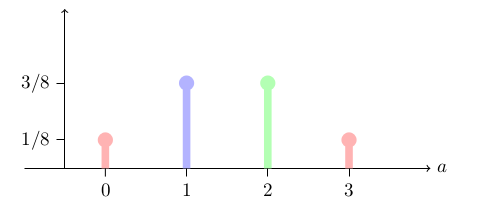
\includegraphics[width=0.9\linewidth]{v2}
	\end{minipage}%
	\begin{minipage}{.5\textwidth}
		\centering
		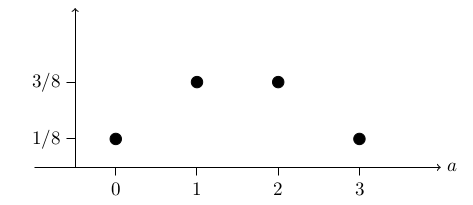
\includegraphics[width=0.9\linewidth]{v3}
	\end{minipage}
\end{figure}
Los gr\'aficos coloreados muestran c\'omo se construye la funci\'on de distribuci\'on acumulativa acumulando la probabilidad como un incremento. Los gr\'aficos en blanco y negro son las presentaciones  est\'andar.
}
\end{frame}

\begin{frame}{Gr\'aficos de $p(a)$ y $F(a)$ (continuaci\'on)}
\begin{figure}
	\centering
	\begin{minipage}{.5\textwidth}
		\centering
		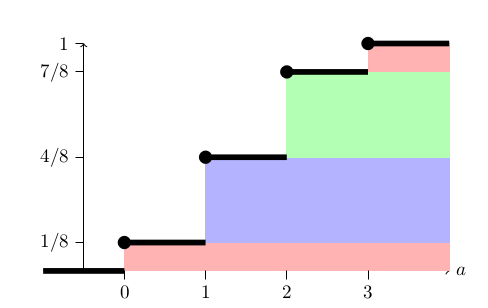
\includegraphics[width=0.8\linewidth]{v4}
	\end{minipage}%
	\begin{minipage}{.5\textwidth}
		\centering
		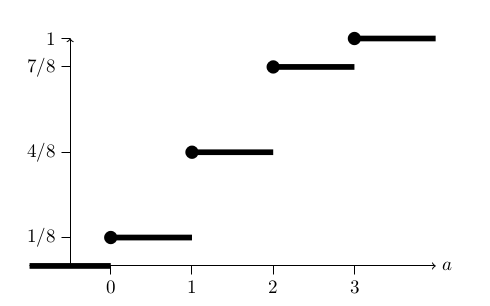
\includegraphics[width=0.8\linewidth]{v5}
	\end{minipage}
\end{figure}

\vspace{0.2cm}

\small {Para el \underline{Ejemplo4}, el PMF y el CDF, est\'a dado por:}
\begin{figure}
	\centering
	\begin{minipage}{.5\textwidth}
		\centering
		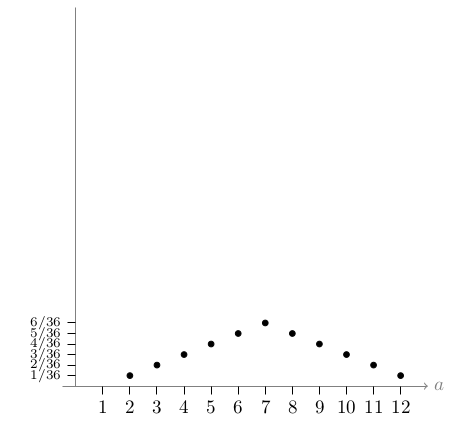
\includegraphics[width=0.7\linewidth]{v6}
	\end{minipage}%
	\begin{minipage}{.5\textwidth}
		\centering
		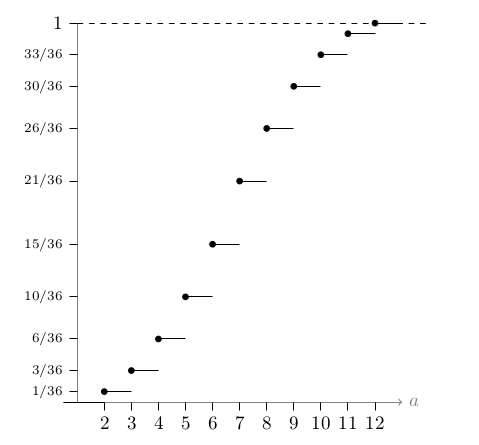
\includegraphics[width=0.7\linewidth]{v7}
	\end{minipage}
\end{figure}
\end{frame}

\begin{frame}{Propiedades de la funci\'on de distribuci\'on acumulativa}
El CDF $F$ de una variable aleatoria satisface varias propiedades:
\begin{itemize}
	\item $F$ es no decreciente. Es decir, su gr\'afico nunca cae, o simb\'olicamente si $a \leq b$ entonces $F(a) \leq F(b)$.
	\item $0 \leq F(a) \leq 1$.
	\item $\lim_{a \rightarrow \infty}F(a) = 1$,\qquad, $\lim_{a \rightarrow -\infty}F(a) = 0$. 
\end{itemize}

\vspace{0.8cm}

\scriptsize{En palabras, (1) dice que la probabilidad acumulativa $F(a)$ aumenta o permanece constante a medida que $a$ aumenta, pero nunca disminuye; (2) dice que la probabilidad acumulada est\'a siempre entre $0$ y $1$; (3) dice que a medida que $a$ se hace muy grande, se hace cada vez m\'as cierto que $X \leq a$ y cuando $a$ se vuelve muy negativo se hace cada vez m\'as cierto que $X> a$.}

\end{frame}

\begin{frame}{Caracter\'istica de la  funci\'on de distribuci\'on acumulativa}

\small {Para una variable aleatoria discreta, $F_X(x)$ tiene la apariencia de escalera. En cada uno de los puntos $x_i$, tiene un salto positivo igual a $p_X(x_i)$. Entre estos puntos, es decir, en el intervalo $[x_i, x_i + 1)$, tiene un valor constante. En otras palabras,  tenemos lo siguiente:
	
	
	\begin{align*}
	F_X(x) &= F_X(x_i)\ \ \text{para}\ \ x_i \leq x < x_{i +1}\\
	F_X(x_{i + 1}) &= F_X(x_i) + p_{X}(x_{i + 1}).
	\end{align*}

Como se muestra en la siguiente figura:

\vspace{0.2cm}

\begin{figure}[ht]
	\centering
	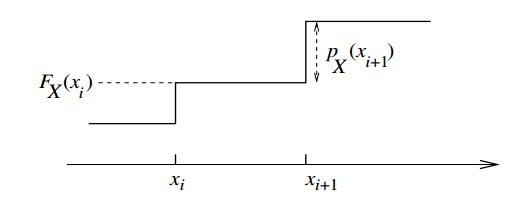
\includegraphics[scale=.35]{v8.png}
\end{figure}
}
\end{frame}

\begin{frame}{Distribuciones espec\'ificas}
	
\textbf{\textcolor{blue}{Distribuci\'on de Bernoulli}}

\underline{Modelo:}  La distribuci\'on de Bernoulli modela ensayos  en un experimento que puede resultar en \'exito o fracaso. Esta es la distribuci\'on m\'as importante y tambi\'en es la m\'as simple. Una variable aleatoria $X$ tiene una distribuci\'on de Bernoulli con  par\'ametro $p$ si:

\begin{itemize}
	\item $X$ toma los valores $0$ 	y $1$.
	\item $\mathbb{P}(X = 1) = p$ y $\mathbb{P}(X = 0 ) = 1- p$.
\end{itemize}


\vspace{0.5cm}


\scriptsize{Escribiremos $X \sim \text{Bernoulli}(p)$ o $\text{Ber}(p)$, que se lee: $X$ sigue una distribuci\'on de Bernoulli con el par\'ametro $p$. Un modelo simple para la distribuci\'on de Bernoulli consiste en lanzar  una moneda con probabilidad $p$ de caras, con $X = 1$ en las caras y $X = 0$ en los sellos. 
	
La terminolog\'ia general es decir que  $X$ es $1$ en los \'exitos y $0$ en los fracasos, con el \'exito y el fracaso definido por el contexto.
}
\end{frame}

\begin{frame}{Distribuciones espec\'ificas}
Aqu\'i se muestran  la tabla y los gr\'aficos del PMF y del CDF para la distribuci\'on de $\textbf{Bernoulli} (1/2)$ 

\begin{figure}
	\centering
	\begin{minipage}{.5\textwidth}
	\begin{table}[]
		\centering
		\begin{tabular}{ccc}
			valor  a  :    & 0    & 1    \\
			PMF   p(a): & 1/2 & 1/2     \\
			CDF   F(a):& 1/2  &  1	
		\end{tabular}
	\end{table}
	\end{minipage}%
	\begin{minipage}{.3\textwidth}
		\centering
		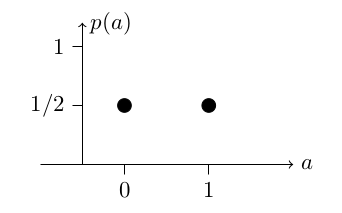
\includegraphics[width=1.2\linewidth]{v9}
	\end{minipage}
		\begin{minipage}{.3\textwidth}
			\centering
			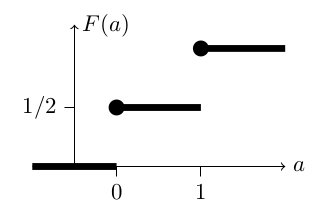
\includegraphics[width=1.2\linewidth]{v10}
		\end{minipage}
\end{figure}

\end{frame}

\begin{frame}{Distribuciones espec\'ificas}
En general los gr\'aficos del PMF y el CDF para una distribuci\'on de Bernoulli, son de la forma:

\begin{figure}
	\centering
	\begin{minipage}{.5\textwidth}
		\begin{table}[]
			\centering
			\begin{tabular}{ccc}
				valor  a  :    & 0    & 1    \\
				PMF   p(a): & 1 -p &  p     \\
				CDF   F(a):& 1 -p  &  1	
			\end{tabular}
		\end{table}
	\end{minipage}%
	\begin{minipage}{.3\textwidth}
		\centering
		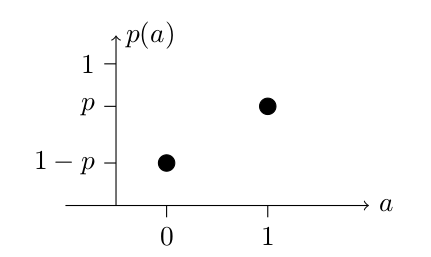
\includegraphics[width=1.2\linewidth]{v11}
	\end{minipage}
	\begin{minipage}{.3\textwidth}
		\centering
		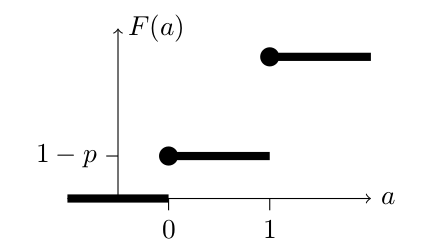
\includegraphics[width=1.2\linewidth]{v12}
	\end{minipage}
\end{figure}
\end{frame}

\begin{frame}{Distribuciones espec\'ificas}
	
\textbf{\textcolor{blue}{Distribuci\'on de Binomial}}

\small{La distribuci\'on $\text{Binomial}(n, p)$, o $\text{Bin}(n, p)$, modela el n\'umero de \'exitos en $n$ ensayos independientes de $\text{Bernoulli}(p)$.

Aqu\'i hay una jerarqu\'ia. Un solo ensayo  de Bernoulli es, digamos, un lanzamiento de una moneda. Un solo ensayo binomial consta de $n$ ensayos de Bernoulli. Para el lanzamiento  de una moneda, el espacio muestral para un ensayo de Bernoulli es $\{H, T\}$. El espacio muestral para un ensayo binomial son todas las secuencias de caras  y sellos de longitud $n$. Del mismo modo, una variable aleatoria de Bernoulli toma los valores $0$ y $1$ y una variable aleatoria binomial toma los valores $0, 1, 2,\dots n$.

\vspace{0.3cm}

\begin{itemize}
	\item \textbf{Ejemplo 7} $\text{Binomial(1,p)}$ es lo mismo que $\text{Bernoulli(p)}$.
	\item \textbf{Ejemplo 8} El n\'umero de caras  en $n$ lanzamientos de una moneda con probabilidad $p$ de caras sigue una distribuci\'on $\text{Binomial}(n, p)$.
\end{itemize}
}
\end{frame}

\begin{frame}{Distribuciones espec\'ificas}
\small{Describimos $X \sim \text{Binomial}(n, p)$ d\'andonos sus valores y probabilidades. Para la notaci\'on usaremos $k$ para indicar un n\'umero arbitrario entre $0$ y $n$.
	
Recordamos que \texttt{n elige k} = $\binom{n}{k}$, es el n\'umero de maneras de elegir $k$ cosas de una colección de $n$ cosas y tiene la f\'ormula

\[
\binom{n}{k} = \frac{n!}{k!(n - k)!}
\]

(Tambi\'en se denomina coeficiente binomial). 

\vspace{0.3cm}

Aqu\'i hay una tabla para la PMF de una variable aleatoria $\text{Binomial}(n, k)$. 

\begin{table}[]
	\centering
	\begin{tabular}{ccccccc}
		valor a : & 0          & 1 &  ... & k & ...& n \\
		PMF p(a): & $(1 -p)^n$ & $\binom{n}{1}p^1(1 -p)^{n -1}$   &...     & $\binom{n}{k}p^1(1 -p)^{n -k}$  & ...& $p^n$   
	\end{tabular}
\end{table}

\vspace{0.2cm}

\textbf{\small{\underline{Ejemplo 9:}}}
?`Cu\'al es la probabilidad de $3$ o m\'as caras en $5$ lanzamientos de una moneda ?.
}
\end{frame}

\begin{frame}{Distribuciones espec\'ificas}
	
\small{ Para concretar, sean $n = 5$ y $k = 2$  (el argumento para valores arbitrarios $n$ y $k$ es id\'entico). Entonces $X \sim \text{Binomial}(5, p)$ y queremos calcular $p(2)$. El largo camino para calcular $p(2)$ es enumerar todas las maneras de obtener exactamente $2$ caras en $5$ lanzamientos  de monedas y sumar sus probabilidades. La lista tiene 10 entradas:
	
CCSSS, CSCSS, CSSCS, CSSSC, SCCSS, SCSCS, SSSSC, SSCCS, SSCSC,
SSSCC
	
Cada entrada tiene la misma probabilidad de ocurrir, a saber:

\[
p^2(1 - p)^3.
\]
}

\scriptsize{Esto se debe a que cada una de las dos caras tiene probabilidad $p$ y cada una de los $3$ sellos tiene probabilidad $1 - p$. Debido a que los lanzamientos individuales son independientes, podemos multiplicar las probabilidades. 
	
Por  tanto, la probabilidad total de exactamente $2$ caras  es la suma de $10$ probabilidades id\'enticas, es decir, $p(2) = 10p^2 (1 - p)^3$, como se muestra en la tabla.
}
\end{frame}

\begin{frame}{Distribuciones espec\'ificas}
\small{Esto nos guia, la manera m\'as corta de hacer el c\'alculo. Tenemos que contar el n\'umero de secuencias con exactamente $2$ caras. Para hacer esto necesitamos elegir $2$ de los lanzamientos para ser caras y los $3$ restantes para ser sellos. El n\'umero de tales secuencias es el n\'umero de formas de  elegir $2$ de $5$ cosas, es decir, $\binom{5}{2}$.
	
Dado que cada secuencia tiene la misma probabilidad, $p^2(1 - p)^3$, obtenemos la probabilidad de exactamente $2$ caras $p(2) = \binom{5}{2}p^2(1 - p)^3$.


\vspace{0.3cm}
	
Aqu\'i algunos gr\'aficos de la  funci\'on de masa de probabilidad binomial}	

\begin{figure}
	\centering
	\begin{minipage}{.3\textwidth}
		%\centering
		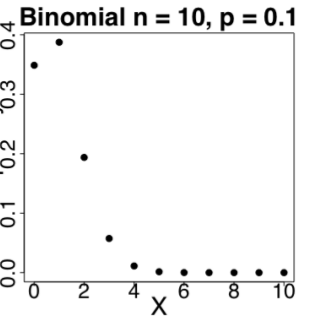
\includegraphics[width=0.8\linewidth]{v13}	
	\end{minipage}
	\begin{minipage}{.3\textwidth}
		\centering
		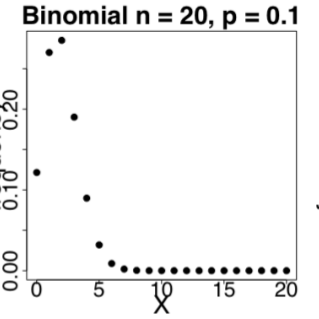
\includegraphics[width=0.8\linewidth]{v14}
	\end{minipage}
	\begin{minipage}{.3\textwidth}
		\centering
		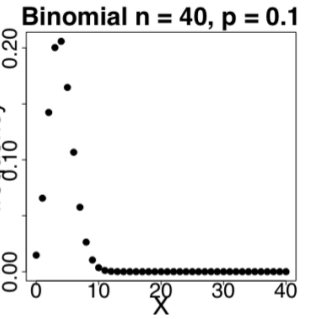
\includegraphics[width=0.8\linewidth]{v15}
	\end{minipage}
\end{figure}
\end{frame}
\begin{frame}{Distribuciones espec\'ificas}
\textbf{\textcolor{blue}{Distribuci\'on geom\'etrica}}

\small{Una distribuci\'on geom\'etrica modela el n\'umero de sellos antes de la primera cara en una secuencia de lanzamientos  de  monedas (ensayos de Bernoulli).
	
\vspace{0.2cm}

\textbf{Ejemplo 10:}
\begin{itemize}
\item \scriptsize{Lanzamos una moneda repetidamente. Sea $X$ el n\'umero de sellos antes de la primera cara. Por lo tanto, $X$ puede ser igual a $0$, es decir, el primer lanzamiento es cara, $1, 2, \dots$. En principio, toma cualquier valor entero no negativo.

\item Damos un lanzamiento de sellos el valor $0$, y de caras  el valor $1$. En este caso, $X$ es el n\'umero de $0$ antes del primer $1$.

\item Damos un lanzamiento de sellos el valor $1$, y de caras  el valor $0$. En este caso, $X$ es el n\'umero de $1$ antes del primer $0$.

\item Llamamos  a un lanzamiento  de sellos un \'exito y de caras un fracaso. Por lo tanto, $X$ es el n\'umero de \'exitos antes de la primer fracaso.

\item Llamamos  a un lanzamiento  de sellos un fracaso y de caras un \'exito. Por lo tanto, $X$ es el n\'umero de fracasos antes de primer \'exito.}
\end{itemize}

\vspace{0.2cm}

\small{Se puede ver estos modelos en muchos escenarios diferentes de este tipo. El lenguaje m\'as neutral es el n\'umero de sellos antes de la primera cara.}
	
}
\end{frame}
\begin{frame}{Distribuciones espec\'ificas}
\small{La variable aleatoria $X$ sigue una distribuci\'on geom\'etrica con par\'ametro $p$ si:
	
\begin{itemize}
	\item $X$ toma los valores $0,1,2, 3, \dots$
	\item El PMF es dado por $p(k) = \mathbb{P}(X = k) = (1 - p)^kp.$
\end{itemize}

Denotamos esto por $X \sim \text{Geometrica(p)}$. En forma de tabla tenemos:

\begin{table}[]
	\centering
	\begin{tabular}{cccccccc}
		valor a : & 0  & 1 &  2 & 3  & ...& k & ...\\
		PMF p(a): & $p$ & $(1 -p)p$  & $(1 -p)^2p$  & $(1 -p)^3p$  & ...& $(1 -p)^kp$&...   
	\end{tabular}
\end{table}

La distribuci\'on geom\'etrica es un ejemplo de una distribuci\'on discreta que toma un n\'umero infinito de valores posibles.	
}
\end{frame}
\begin{frame}{Distribuciones espec\'ficas}
\small{Las cosas pueden ser confusas cuando trabajamos con \'exitos y fracasos, ya que tal vez queramos modelar el n\'umero de \'exitos antes del primer fracaso o quiz\'as queramos el n\'umero de fracasos antes del primer \'exito. Para mantener las cosas rectas directamente se puede traducir al lenguaje neutral del n\'umero de sellos antes de la primeras caras.
		
\begin{figure}
	\centering
	\begin{minipage}{.5\textwidth}
		\centering
		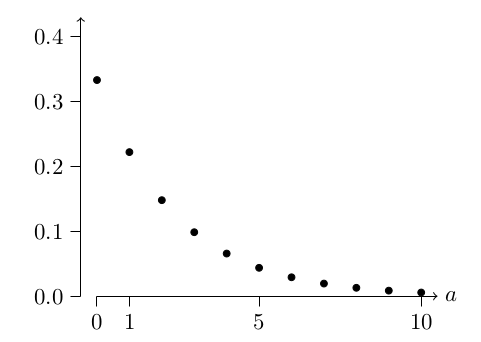
\includegraphics[width=0.7\linewidth]{v16}
	\end{minipage}%
	\begin{minipage}{.5\textwidth}
		\centering
		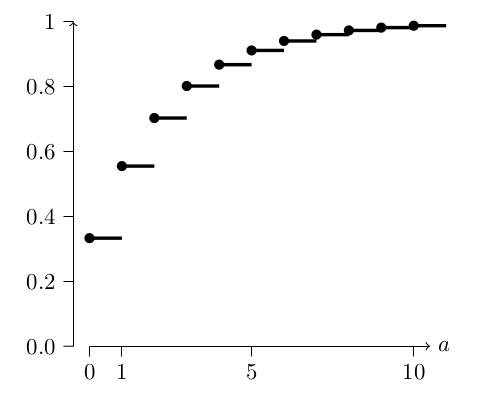
\includegraphics[width=0.7\linewidth]{v17}
	\end{minipage}
\end{figure}

El gr\'afico muestra el PMF y el CDF de la distribuci\'on \texttt{Geometrica(1/3)}.	
}
\end{frame}

\begin{frame}{Distribuciones espec\'ificas}
	\small{
\textbf{Ejemplo 11:}

Supongamos que los habitantes de una isla planean a sus familias teniendo beb\'es hasta que nazca la primera ni\~na. Supongamos que la probabilidad de tener una ni\~na con cada embarazo es de $0.5$ independiente de otros embarazos, que todos los beb\'es sobreviven y no hay nacimientos m\'ultiples. ?`Cu\'al es la probabilidad de que una familia tenga $k$ hijos?.}

\vspace{0.8cm}

\scriptsize{Otra definici\'on com\'un para la distribuci\'on geom\'etrica es el n\'umero de lanzamientos hasta las primeras caras. En este caso $X$ puede tomar el valor de $1$, es decir, el primer lanzamiento es cara, $2, 3,\dots$.  Esta es s\'olo nuestra variable aleatoria geom\'etrica m\'as $1$. 
	
}
	
\end{frame}

\begin{frame}{Distribuciones  espec\'ificas}

\textbf{\textcolor{blue}{Distribuci\'on uniforme discreta}}

La distribuci\'on uniforme discreta modela cualquier situacion en la que todos los resultados sean igualmente probables.

\[
X \sim \text{Uniforme(N)}.
\]

\vspace{0.2cm}

$X$ toma los valores $1, 2, 3,\dots, N$, cada una con probabilidad $1/ N$. Ya hemos visto esta distribuci\'on muchas veces cuando modelamos monedas  ($N = 2$), dados ($N = 6$), cumplea\~nos ($N = 365$) y manos de p\'oquer ($N = \binom{52}{5}$).
\end{frame}

\begin{frame}{Aritm\'etica con variables aleatorias}
	
\small{Podemos hacer aritm\'etica con variables aleatorias. Por ejemplo, podemos sumarlas, multiplicarlas o elevarlas al cuadrarlo.

Hay una idea simple, pero extremadamente importante para contar. Esta dice que si tenemos una secuencia de n\'umeros que son $0$ o $1$ entonces la suma de la secuencia es el n\'umero de unos.}


\scriptsize{\textbf{Ejemplo 12:}
Consideramos la secuencia con $5$ unos

1, 0, 0, 1, 0, 0, 0, 1, 0, 0, 0, 0, 1, 0, 0, 0, 1, 0, 0.

Es f\'acil ver que la suma de esta secuencia es 5 el n\'umero de unos.

Ilustramos esta idea contando el n\'umero de caras en $n$ lanzamientos de una moneda.}

\textbf{Ejemplo 13:}

\scriptsize{Lanzamos una moneda $n$ veces. Sea $X_j$ es 1 si el j-\'esimo lanzamiento es cara y $0$ si es sello. Entonces, $X_j$ es una variable aleatoria de $\text{Bernoulli}(1/2)$.

Sea X el n\'umero total de caras en los $n$ lanzamiento. Asumiendo que  los lanzamientos son independientes, sabemos que  $X \sim \text{Binomial}(n, 1/2)$. Tambi\'en podemos escribir:

\[
X = X_1 +X_2 +X_3 + \dots + X_n.
\]
}
\end{frame}

\begin{frame}{Aritm\'etica con variables aleatorias(continuaci\'on)}
\small{De nuevo, esto se debe a que los t\'erminos de la suma a la derecha son todos $0$ o $1$. Por lo tanto, la suma es exactamente el n\'umero de $X_j$ que son 1, es decir, el n\'umero de caras.
	
Lo importante a ver en el ejemplo anterior es que hemos escrito la variable aleatoria binomial $X$, m\'as complicada, como la suma de variables aleatorias extremadamente simples $X_j$.  Esto nos permitir\'a manipular $X$ algebraicamente.

\textbf{Ejemplo 14:}

Supongamos $X$ e $Y$ son variables aleatorias independientes con las siguientes tablas:


\begin{table}[]
	\centering
	\begin{tabular}{c|c c c c c c}
		%\hline
		Valores de  X & x:       & 1    & 2    & 3    & 4  &   \\ \hline
		PMF           & $p_X(x)$: & 1/10 & 2/10 & 3/10 & 4/10 \\ 
		Valores de Y  & y:       & 1    & 2    & 3    & 4   & 5  \\ \hline
		PMF           & $p_Y(y)$:   & 1/15 & 2/15 & 3/15 & 4/15 & 5/15 \\ 
	\end{tabular}
\end{table}
}
\end{frame}

\begin{frame}{Continuaci\'on del ejemplo}
	
\small{Comprueba que la probabilidad total para cada variable aleatoria es $1$. Construye  una tabla para la variable aleatoria $X + Y$.
	
\vspace{0.5cm}


\textbf{\textcolor{blue}{Respuesta:}}

Lo primero que debemos hacer es una tabla bidimensional para el espacio  muestral del producto que consiste en pares $(x, y)$, donde $x$ es un valor posible de $X$ e $y$ uno de $Y$.

Para ayudar a hacer el c\'alculo, las probabilidades para los valores de $X$ se ponen en la columna de la derecha y las de $Y$ se encuentran en la fila inferior. Dado que $X$ e $Y$ son independientes, la probabilidad para el par $(x, y)$ es s\'olo el producto de las probabilidades individuales.	
}
\end{frame}

\begin{frame}{Continuaci\'on del ejemplo(1)}
\small{

En el siguiente gr\'afico, las rayas diagonales muestran conjuntos de cuadrados donde $X + Y$ es el mismo. Todo lo que tenemos que hacer para calcular la tabla de probabilidad para $X + Y$ es sumar las probabilidades para cada raya.}

	
\begin{figure}[ht]
	\centering
	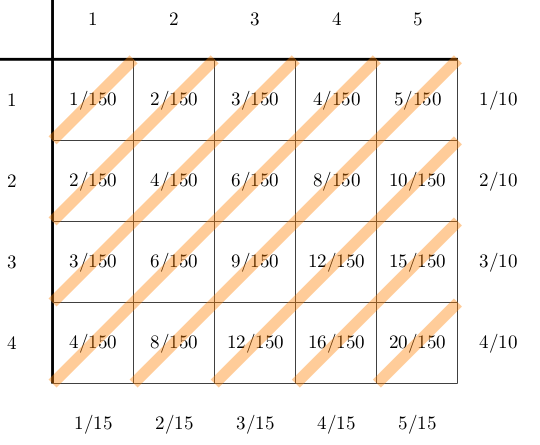
\includegraphics[scale=.3]{v18.png}
\end{figure}

 \scriptsize{
\begin{table}[]
	\centering
	\begin{tabular}{ccccccccc}
		Valores de X + Y : & 2     & 3     & 4      & 5      & 6      & 7      & 8      & 9      \\
		PMF                & 1/150 & 4/150 & 10/150 & 20/150 & 30/150 & 34/150 & 31/150 & 20/150
	\end{tabular}
\end{table}
}
\end{frame}

\end{document}